\section{Modeling the Bridge Using mCRL2}

With the requirements clearly stated, now the bridge can be modeled. In order to create a model that can be verified using $\mu$-calculus, the mCRL2 program can be used. The code for the model can be found in \ref{sec:mcrl} or the attached file \texttt{Bridge\_group7.mcrl}.

When writing the code, we kept to the architecture from section \ref{sec:act} including three processes. The \emph{signs} process communicates with the \emph{barriers} process, which in turn communicates with the \emph{bridge} process. This leads to a linear structure of the model, as shown in figure \ref{fig:graph} and \ref{fig:view}.
%
\begin{figure}[htb]
\centering
		\begin{subfigure} [h] {0.3\textwidth}
		\centering
		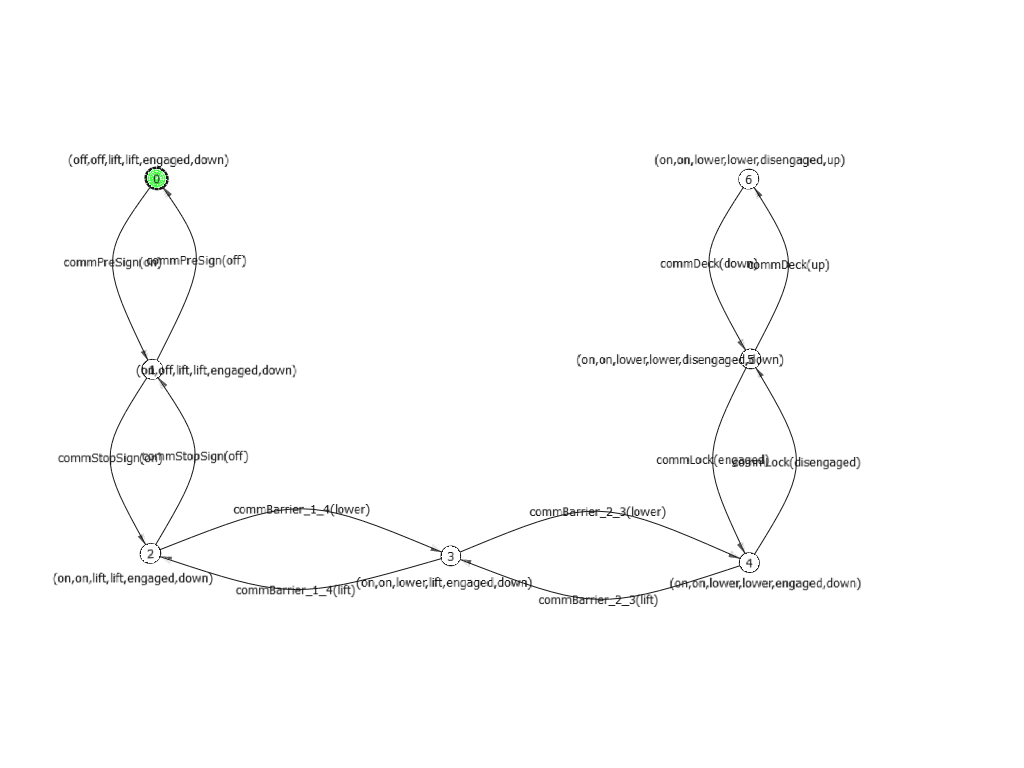
\includegraphics[width=150px]{Images/Bridge_ltsgraph.png}
		\caption{Graph made by \texttt{ltsgraph}}
		\label{fig:graph}
	\end{subfigure}
\hspace{5em}
	\begin{subfigure} [h] {0.3\textwidth}
		\centering
		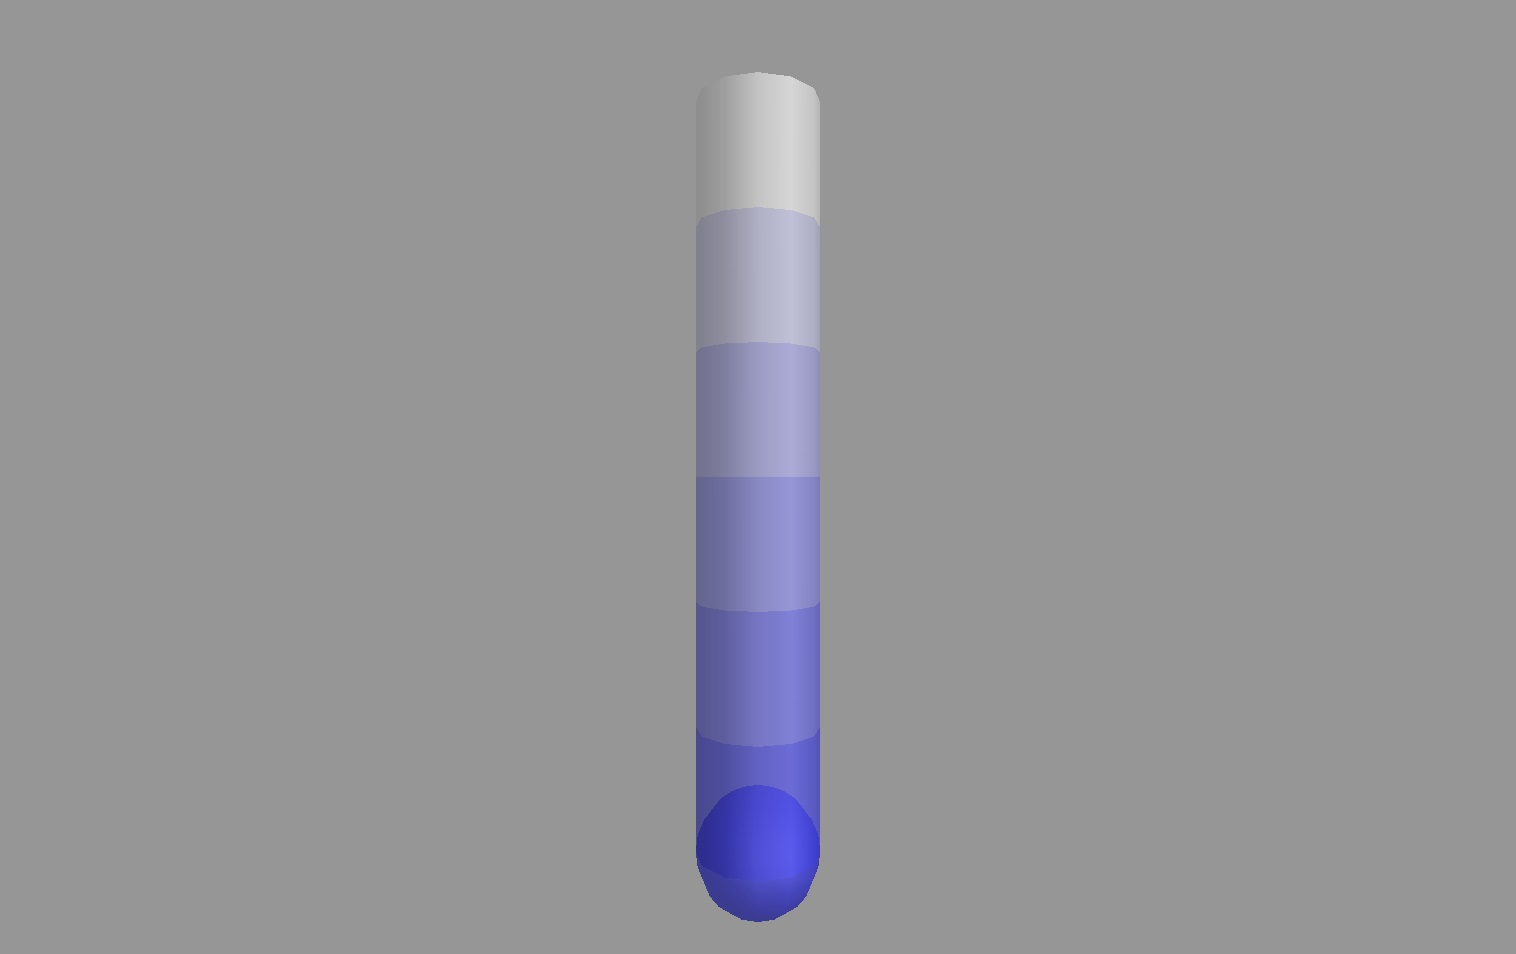
\includegraphics[width=150px]{Images/Bridge_ltsview.jpg}
		\caption{Image made by \texttt{ltsview}}
		\label{fig:view}
	\end{subfigure}
\caption{Graphical interpretations of the Bridge model.}%
\label{}%
\end{figure}%
%